%%%%%%%%%%%%%%%%%%%%%%%%%%%%%%%%%%%%%%%%%%%%%%%%%%%%%%%%%%%%%%%%%%%%%%%%%%%%%%%%
%2345678901234567890123456789012345678901234567890123456789012345678901234567890
%        1         2         3         4         5         6         7         8

\documentclass[letterpaper, 10 pt, conference]{ieeeconf}  % Comment this line out
                                                          % if you need a4paper
%\documentclass[a4paper, 10pt, conference]{ieeeconf}      % Use this line for a4
                                                          % paper

\IEEEoverridecommandlockouts                              % This command is only
                                                          % needed if you want to
                                                          % use the \thanks command
\overrideIEEEmargins
% See the \addtolength command later in the file to balance the column lengths
% on the last page of the document



% The following packages can be found on http:\\www.ctan.org
\usepackage{graphicx} % for pdf, bitmapped graphics files
%\usepackage{epsfig} % for postscript graphics files
%\usepackage{mathptmx} % assumes new font selection scheme installed
%\usepackage{times} % assumes new font selection scheme installed
%\usepackage{amsmath} % assumes amsmath package installed
%\usepackage{amssymb}  % assumes amsmath package installed

\title{\LARGE \bf
BIF 701 LAB 8: Secondary Structure Prediction
}

%\author{ \parbox{3 in}{\centering Huibert Kwakernaak*
%         \thanks{*Use the $\backslash$thanks command to put information here}\\
%         Faculty of Electrical Engineering, Mathematics and Computer Science\\
%         University of Twente\\
%         7500 AE Enschede, The Netherlands\\
%         {\tt\small h.kwakernaak@autsubmit.com}}
%         \hspace*{ 0.5 in}
%         \parbox{3 in}{ \centering Pradeep Misra**
%         \thanks{**The footnote marks may be inserted manually}\\
%        Department of Electrical Engineering \\
%         Wright State University\\
%         Dayton, OH 45435, USA\\
%         {\tt\small pmisra@cs.wright.edu}}
%}

\author{Christopher Eeles% <-this % stops a space
}

\begin{document}

\maketitle
\thispagestyle{empty}
\pagestyle{empty}

%%%%%%%%%%%%%%%%%%%%%%%%%%%%%%%%%%%%%%%%%%%%%%%%%%%%%%%%%%%%%%%%%%%%%%%%%%%%%%%%
\begin{abstract}

This laboratory will utilize the NCBI Nucleotide Database to access the FASTA sequence of the HHV-1 and HHV-2 associated RNA molecule LAT. The FASTA will then be input into the mFold secondary structure prediction tool to generate images of potential LAT configurations. These images will be compared to identify significantly different 2D arrangements, which will be analyzed to infer how secondary structure may contribute to stablility of LAT molecules within HHV infected host cells.

\end{abstract}

%%%%%%%%%%%%%%%%%%%%%%%%%%%%%%%%%%%%%%%%%%%%%%%%%%%%%%%%%%%%%%%%%%%%%%%%%%%%%%%%
\section{INTRODUCTION}

The human herpes viruses---HHV-1 and HHV-2---most commonly infect oral or genital epithelial cells, generating inflammatory lesions.$^5$ While symptoms tend to be acute in nature, viral infection is lifelong due to the transport of HHV particles into the ganglia of local sensory neurons.$^2^,^6$ Within these neurons, the virus enters latency where it remains dormant until some environmental factor triggers recurrence.$^2^,^6$ Investigation of the cause and mechanism of recurrence is still preliminary, but an RNA molecule known as latency-associated transcript (LAT) is suspected to play a role.$^6$ Concentration of the LAT molecule within asymptomatic host neurons were found to be significantly higher in comparison to symptomatic ones, leading to the hypothesis that LAT plays a role in suppressing expression of the HHV genome.$^6$ 

If this is the case, the stability of LAT RNA within host host cells could be an important modulator of reinfection, thus constituting a molecule of interest in HHV pathophysiology as well as a potential target for pharmaceutical intervention.$^6$ In this laboratory we will be utilizing web-based secondary structure prediction tools to uncover possible configurations of LAT based on its primary sequence. This information will be used to evaluate the role secondary structure plays in stabilization of LAT within the RNase rich environment of the host cell cytosol.$^1$ If meaningful conclusions can be drawn, they may enable development of compounds to stabilize LAT or identification of enzymatic pathways which lead to its degradation and thus re-manifestation of HHV pathology.$^6$ Such discoveries could inform new lines of research on HHV and better elucidate the mechanism by which recurrence is triggered.

\section{METHODS}

\subsection{NCBI Nucleotide Database}

Access to the NCBI Nucleotide Database is available at https://www.ncbi.nlm.nih.gov/nucleotide/. The service provides an integrated search query across major nucleotide databases including NCBIs own nucleotide database and GenBank divisions storing expressed sequence tags (EST) and genome sequence survey (GSS) data.$^3$ In this lab we used it to identify the whole genome of HHV-1, from which we extracted the FASTA file for the LAT intron. Before saving the file, the 'reverse complement' option was disabled to yield the DNA version of the RNA transcript.

\subsection{mFold}

Access to the mFold tool is available at http://unafold.rna.albany.edu/?q=mfold. The web service was developed by Michael Zucker, a professor of mathematics at Rensselaer Polytechnic Institute, and is used to predict secondary structures from primary sequence data utilizing a mainly thermodynamic model.$^4$ After navigating to the mRNA folding form we copied the curated FASTA file from NCBI into the sequence text box and clicked format to convert it from DNA to RNA. The formatting resulted in an error, but clicking through and switching to 'A batch' under the select option and entering an email allowed submission of the job. Results of this search were downloaded as PDF files and manually compared to generate the figures in the RESULTS section.

\section{RESULTS}

\begin{figure}[h]
    \centering

    \fbox{
        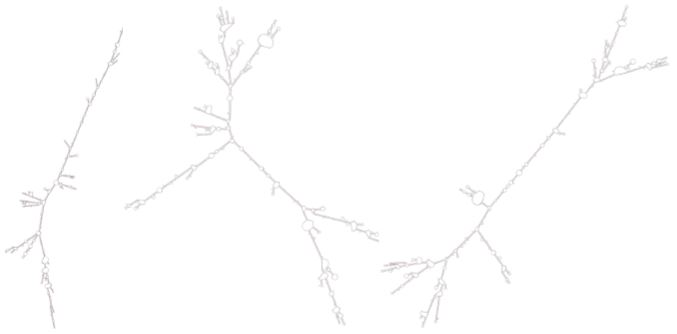
\includegraphics[width=3in]{Fig1.JPG}
    }
    \caption{Left = 'The Curve', Middle = 'The Man', Right = "The Stick"}
\end{figure}
\begin{figure}[h]
    \centering

    \fbox{
        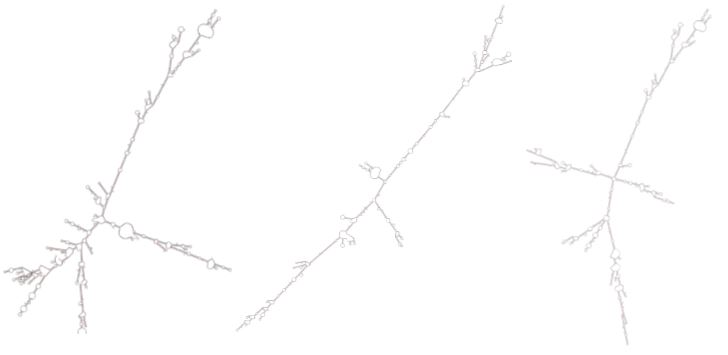
\includegraphics[width=3in]{Fig2.JPG}
    }
    \caption{Left = 'The Tripod', Middle = 'The Y', Right = "The Cross"}
\end{figure}

After manual comparison of the 36 pdf images generated from mFold, six significant structures were selected and recorded in Fig. 1. Use of an image comparison algorithm would have expedited the process, but was decided against due to lack of technical expertise. The output from mFold includes bond colourization, indicating the confidence level for each base pairing within a given secondary structure.

\section{DISCUSSION AND CONCLUSION}

The results demonstrated that there are a wide range of secondary structures which LAT could display. Closer examination of the subset selected for the results section revealed that hairpin and internal loops are the most prevalent motifs within each respective configuration.$^2$ Bulge motifs were also observed but seem, at least for this primary sequence, to be less frequent.$^2$ Pseudo knots were not present in our results, unless you count some terminal hairpin loops which are in close proximity; this result makes sense considering that inter motif interactions are likely a more significant contributor to tertiary than secondary structure.$^2$ Interestingly, the nucleotide motifs displayed a fractal like pattern wherein larger loops split the molecule into one or more branches, which then spawned smaller loops repeating the branching pattern---although less frequently with each subsequent branching. The ends of each branch terminated in one or more hairpin loop structures, often directly branching off the loop proximal to them. 

Base pairing was more prevalent than any of the non-paired structural motifs and the majority of the bonds were red, indicating a high degree of confidence in each respective pairing within the predicted configuration.$^2$ While the overall molecular topology displayed several distinct patterns, all samples displayed a similar pattern of motifs and branching, with variations tending to occur in the number or location of the three to five primary branches off the molecule.$^2$ Overall, the 36 structures predicted via mFold displayed more similarities than differences and fell within a few slightly varied primary branching patterns with smaller variations in overall length and sub-branching from each of the parent branches. Explorations of tertiary structure via crystallization or NMR may be able to limit the number of possible secondary structural configurations by eliminating those inconsistent with the known tertiary structure; such an approach may allow convergence on high confidence secondary structures via bottom up and top down structural studies.

Considering the stability of the LAT molecule within host cells, the relative frequency of double stranded vs single stranded RNA residues within the molecule are likely a deciding factor. Single stranded mRNA is transported to the ribosome bound to carrier proteins, and once translation completes, the bare single stranded mRNA is quickly degraded by RNases to be recycled in future transcriptions. Given that RNases themselves, as well as other molecules such as tRNA, are composed primarily of double stranded RNA, the stability of double stranded LAT seems to stem from the inability of cells to target dsRNA without interupting their own cellular processes. However, even ribozymes tend to be short lived in the cytosol relative to proteins and therefore additional factors are needed to account for the consistently high concentration of LAT in the host neurons of asymptomatic individuals. Two potential mechanisms spring to mind. Firstly, the genome of HHV, once integrated into the host cells genome, may contain an element leading to continuously high transcription of the LAT intron and therefore the rate of production compensates for the rate of degradation. Secondly, the LAT molecule may iteslf display ribozyme activity which slows its degradation in the cytosol. Either or both of these mechanisms could explain the stability of the LAT molecule, but further study is necessary to substantiate such hypotheses.

Reflecting on these analyses it seems that secondary structure is indeed a factor in the stability of LAT---and similar dsRNA molecules and ribozymes---within the host neurons, and cells more generally. Further investigation of the activity of LAT itself, or the enzymes which result in its degradation, could yield new insights into the pathways by which its concentration decreases in recurrent HHV infections. Understanding such pathways could help identify targets for pharmaceutical intervention to increase the stability of LAT within infected host cells, either directly by re-enforcing its stability or indirectly by inhibiting enzymes which degrade it. However, given the numerous other essential dsRNA molecules within host cels it is important to ensure any intervention does not affect the function or concentration of these molecules. 

Even if LAT is found to only be correlated with HHV recurrence, studying the pathways adjacent to it could provide useful information for discerning the causal factors. Therefore secondary structure prediction is a field with the potential to contribute significantly to understanding the role of nucleotide secondary structure in the function of non-mRNA transcripts. Moreover, such contributions may enable advances in the biochemical and physiological understanding of the pathways in which these molecules are involved, eventually enabling identification of new molecular targets for medical interventions in a wide range of pathologies. Given the computational nature of structure prediction problems, bioinformaticians have a key role to play in such advances and thereby can contribute significantly to the rate of innovation in the medical and pharmaceutical industries. Opportunities such as these make bioinformatics an exciting area of biomedical, as well as basic biological, research and the growth of this field will undoubtedly benefit both those employed in it and society writ large.

\addtolength{\textheight}{-12cm}  % This command serves to balance the column lengths
                                  % on the last page of the document manually. It shortens
                                  % the textheight of the last page by a suitable amount.
                                  % This command does not take effect until the next page
                                  % so it should come on the page before the last. Make
                                  % sure that you do not shorten the textheight too much.

%%%%%%%%%%%%%%%%%%%%%%%%%%%%%%%%%%%%%%%%%%%%%%%%%%%%%%%%%%%%%%%%%%%%%%%%%%%%%%%%

\begin{thebibliography}{99}

\bibitem{c1} School of Biological Sciences and Applied Chemistry. (2018). BIF701 Lab 8: Secondary Structure Prediction. Seneca College: Toronto, ON.
\bibitem{c2} School of Biological Sciences and Applied Chemistry. (2018). BIF 701 Topic 8: Secondary Structure Prediction. Seneca College: Toronto, ON. 
\bibitem{c3} Cooper P, Landrum M, Mizrachi I, et al. (2010) Entrez Sequences Quick Start. In: Entrez Sequences Help [Internet]. National Center for Biotechnology Information: Bethesda, MD. Retrieved from: https://www.ncbi.nlm.nih.gov/books/NBK44863/
\bibitem{c4} Michael Zuker \& Nick Markham. (2018). mFold Web Server. In The RNA Institute [Internet]. State University of New York: Albany, NY. Retrieved from http://unafold.rna.albany.edu/?q=node/60
\bibitem{c5} Whitley R, Kimberlin DW, Prober CG. Pathogenesis and disease. Human Herpesviruses Chapter 32: Biology, Therapy, and Immunoprophylaxis. Cambridge: Cambridge University Press. Retrieved from https://www.ncbi.nlm.nih.gov/books/NBK47449/
\bibitem{c6}Nicoll MP, Hann W, Shivkumar M, Harman LER, Connor V, et al. (2016) The HSV-1 Latency-Associated Transcript Functions to Repress Latent Phase Lytic Gene Expression and Suppress Virus Reactivation from Latently Infected Neurons. PLOS Pathogens 12(4): e1005539. https://doi.org/10.1371/journal.ppat.1005539

\end{thebibliography}

\end{document}